\chapter{Methods and Characterisation}

\section{Optical CT Materials and Methods}
\label{sec:opticalCTmeth}
The optical CT system is used for two applications; tissue imaging and dosimetry using the solid radiochromic gel PRESAGE. The system is broadly the same for both applications, with some minor hardware changes. The high-quality and uniform dosimetric samples were used to help develop the system and scanning procedure for imaging the more heterogeneous tissue samples.

50 \si{\um} 360 \si{\degree}

\subsection{Hardware}
The  optical CT system is area-detector based, allowing for fast 3-D scanning. A CMOS (complementary metal-oxide semiconductor) camera (Zyla sCMOS, Andor Technology PLC, Belfast, UK) with a large pixel array and fast frame-rate allows for much faster imaging with larger projection matrix size than previously reported systems. Advances in CMOS and CCD (charge-coupled device) camera technology means that higher quality optical CT systems can be built cheaply.  A new PC with 256 GB RAM (Dell), controls acquisition and performs reconstruction, meaning that scans can be carried out much faster. 

Two illumination sources are used, depending on the application. A flat-panel red light-emitting diode (LED) 
(PHLOX-LEDR-BL-100x100-S-Q-1R-24V, Phlox, Aix-en-Provence, France), with a wavelength of 633 nm provides uniform lighting appropriate for imaging PRESAGE\texttrademark , a radiochromic plastic which has a strong absorption peak at 632 nm. 
For tissue imaging the wavelength most appropriate for each sample is provided through the use of a  new broadband white light source (SugarCUBE LED Illuminator, Nathaniel Group Inc., VT, USA) and tunable filter (VariSpec, PerkinElmer, Inc., MA, USA). 


	\begin{figure}
	\centering
	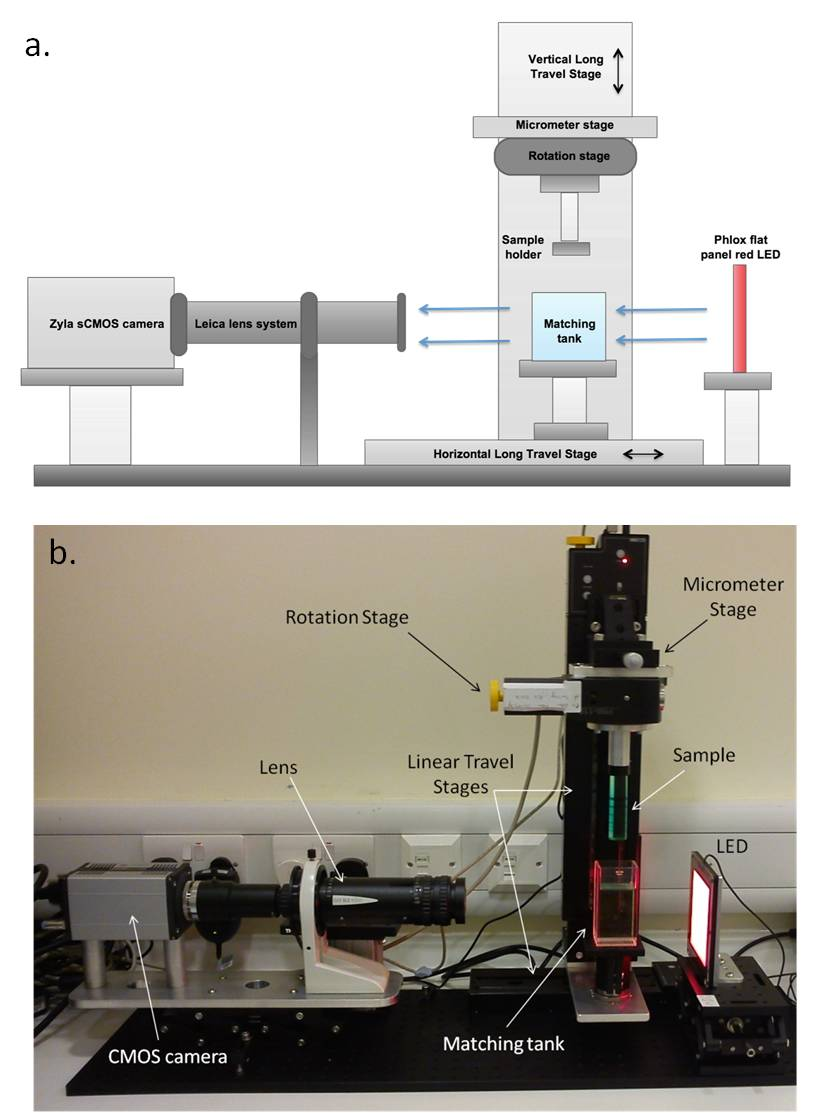
\includegraphics[width = \textwidth]{meth_img/Dosimetry_setup}
	\caption{Diagram and picture  of current set-up of optical CT system at the ICR with principal parts of apparatus labelled. CHANGE picture and add mounts.}
	\label{fig:setup_pic}
	\end{figure}

Samples are suspended from a rotary stage (PRS-110 ZSS43, PI miCos GmbH, Eschbach, Germany) in a glass matching tank (Part 704-002-40-10, Hellma GmbH, M\"{u}llheim, Germany). 
The matching tank is filled with `matching liquid' with a refractive index (RI) close to that of the sample, avoiding refraction at the sample surface. %For PRESAGE samples this matching fluid was a solution of (97\% ethyl hexyl salicylate and 3\% 4-methoxycinnamic acid 2-ethylhexyl ester) giving the same refractive index as the PRESAGE\textregistered. The clearing solution used for each tissue sample was used for matching fluid.
%Add to individual sections

For initial measurements  the rotation stage was supported on a large optical post. In an updated system this post was replaced with an Integrated Long Travel Stage (LTS-300/M, Thorlabs Ltd., Ely, UK ) which allows  accurate and reproducible vertical positioning of samples. 
In collaboration with the ICR workshop, a novel mounting system has been developed to give reproducible positioning of samples allowing pre- and post-irradiation scans of dosimetry gels (see Figure~\ref{fig:Presage_sample_mounts}). 
Two custom sample mounts are used for dosimetry and tissue samples respectively. The dosimetry mount fits caps that are fixed to PRESAGE\textregistered \ samples, meaning the samples are in the same orientation for every scan. 


\begin{figure}
\centering
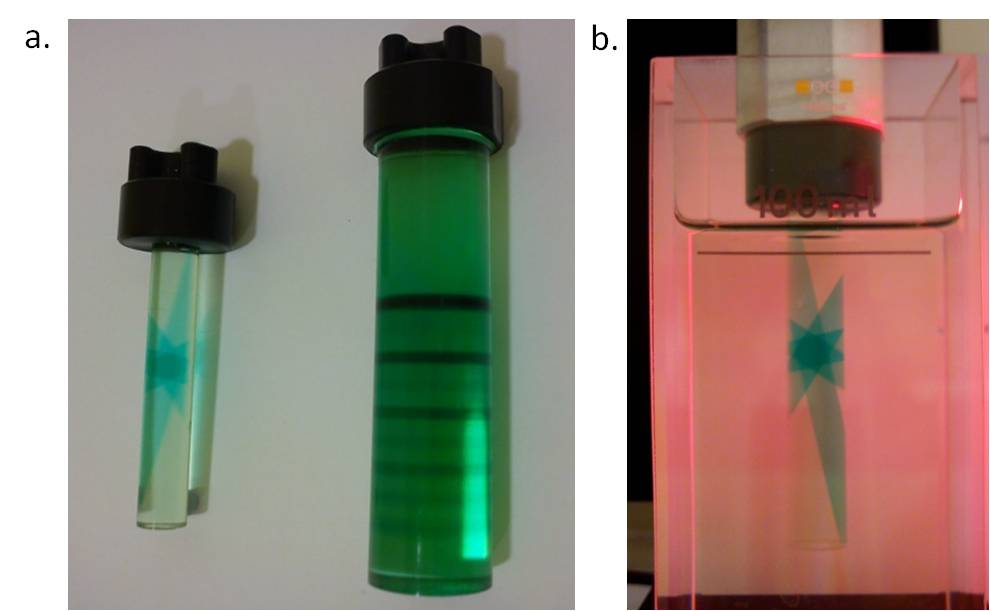
\includegraphics[width=0.9\linewidth]{meth_img/Presage_sample_mounts}
\caption{a. PRESAGE\textregistered \ samples with novel mounts. b. PRESAGE\textregistered \ sample mounted to the rotation stage in the matching tank.}
\label{fig:Presage_sample_mounts}
\end{figure}



The rotation stage is mounted on a micrometer stage allowing  precise alignment of the centre-of-rotation (COR) with the centre of the projection images. If the COR is not aligned with the central pixel column, then the sample will appear to drift across the screen and projection data will not be consistent for all angles. \cite{Oldham:2006b}
The tissue mount has two additional stages, giving the flexibility to position irregular samples on the COR independently of moving the COR.   
An additional Long Travel Stage (LTS-150/M, Thorlabs LTD., Ely, UK ) allows accurate positioning of the sample and tank along the optical axis.  

\begin{figure}
\centering
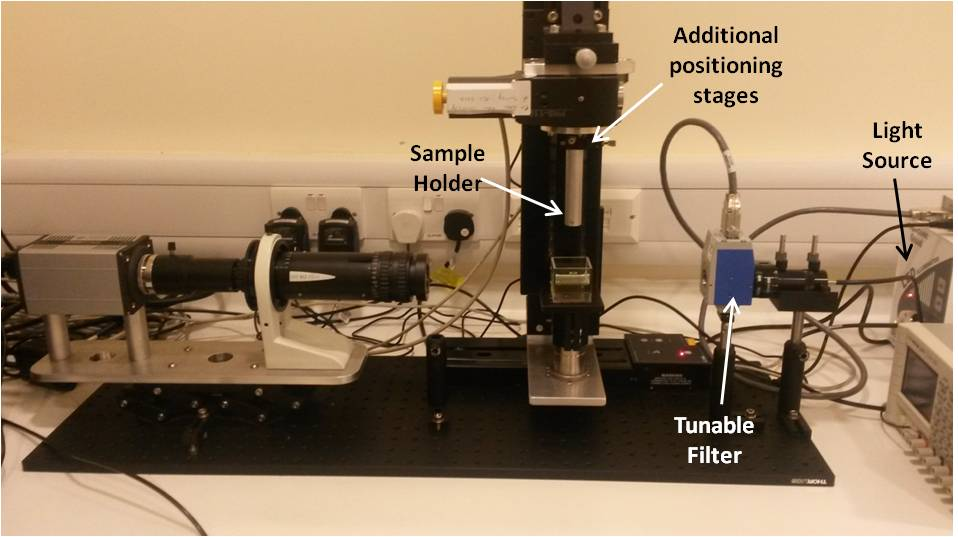
\includegraphics[width=\linewidth]{meth_img/tissue_setup}
\caption{Tissue setup}
\label{fig:tissue_setup}
\end{figure}


Light is collected by an imaging lens system made up of  components of the modular `Z16 APO' zoom system  (Leica Microsystems GmbH, Wetzlar, Germany, see \cite{Doran:2010hn} for details). The use of the zoom lens allows manual adjustment of the focus, depth-of-field and magnification. In general the manual focus was left constant and the LTS stage was used to position the sample and tank along the optical axis for focusing which allows for more repeatable imaging. The procedure for finding the focal position is given  in Section~\ref{sec:focalpos}.








\subsection{Software}
\subsubsection{Acquisition}




Image acquisition and sample rotation are controlled synchronously  by PC using an in-house program written in LabView (National Instruments Corporation Ltd., Berkshire, UK). The high capacity of the PC and camera allows for fast read-out of images giving much reduced scan times to others previously reported. 

Projections can be acquired in two modes. Fast scans are performed in `Continuous' mode, with the sample rotating through $180^{\circ}$ at constant velocity and the camera acquiring projections with a fixed frame rate. This method of scanning is only possible because of the large RAM on the computer. 

If averaging of several projections is necessary to improve the signal-to-noise ratio (SNR) then a `Step and shoot' procedure is used in which the sample is rotated by a fixed angle, several images are acquired, averaged and saved before the sample is rotated again. This scan takes much longer however may be necessary in cases where on-camera binning is not used. 


`Dark' field (DF) and `light' field (LF) images are acquired for each scan, to correct for structural noise in the camera and non-uniformities in the light path respectively. In general 30 DF (with cap on camera) and LF (no sample present) images are averaged. 




Include algorithms? Maybe in appendix?

\subsubsection{Reconstruction}
Reconstruction is carried out via Filtered Back-projection (FBP) incorporating  `correction scans', using in-house software  written by  SJD in IDL (Excelis Visual Information Solutions, Boulder, CO) (see \cite{doranestablishing2013}). LF and DF corrections are applied during reconstruction according to  equation (4) of Krstaji\'{c} \cite{Krstajic:2007ec}.  
%Shepp-Logan filter used?


The software  allows for manual correction of off-axis COR, which commonly changes with height can is very difficult to exactly align mechanically to sub-pixel accuracy. This correction works by simply shifting pixels from one side of the sinogram to the other [CHECK!!]. 

A ring artefact correction has been added to the reconstruction, based on [INSERT reference]. The number of pixels can be chosen depending on the matrix size of the projections. Ring artefacts arise from the presence of a fixed abnormality in the projections which is constant for all angles. They are lines in the projections and can be removed through simple averaging. [ADD DETAILS]


\subsection{Scanning procedure}

The rotation stage and matching tank are positioned in the centre of the focal plane, using the optical axis positioning stage (see Section~\ref{sec:focalpos}).

The magnification is chosen such that the widest part of the sample fits within the  field-of-view (FOV). The projection image matrix size is chosen depending on the required resolution of the final images. Larger matrix projections take longer to acquire and reconstruct. On-camera binning is available which improves SNR of projection images and gives smaller matrix projections covering the entire FOV.

The depth-of-field (DOF) can be adjusted using an aperture in the lens system. The aperture setting will depend on the desired DOF and resolution trade-off (see Section~\ref{subsec:spat_res}).

The light-source intensity is adjusted, avoiding saturation of the  light-field correction images. This intensity will depend on the magnification, camera binning and aperture settings. 

Before image acquisition, the alignment of the COR with the centre of the FOV can be corrected using a LabView program which compares projections at $0^{\circ}$ and $180^{\circ}$. Off-centre COR leads to artefacts which can be corrected as part of the reconstruction. 
Once the COR is correct, samples using the tissue mount, with additional micrometer positioning stages, can  be positioned in the middle of the FOV.

The number of projections depends on the projection matrix size and is calculated using Nyquist sampling condition,
\begin{equation}
N_{proj} = \frac{\pi}{2} N_{pix}
\end{equation} 
where $N_{proj}$ is the number of projections and $N_{pix}$ is the number of projection matrix pixels in the plane orthogonal to the vertical axis.


Projections are then acquired in either `Continuous' or `Step-and-shoot' mode, depending on application. Light and dark field images are acquired afterwards with identical imaging parameters and reconstructed images are produced using IDL software. 








\subsection{Tissue sample preparation}



Before imaging, tissue samples must undergo a series of preparation steps:
\begin{itemize}
	\item Fix in $70\%$ ethanol in phosphate-buffered saline (PBS) overnight
	\item Embed in $0.75\%$ agarose for stability
	\item $3-4$ washes of $100\%$ ethanol
	\item Washes of $30\%$ and $70\%$ 1:2 benzyl benzoate:benzyl alcohol (BABB) in ethanol
	\item $1-2$ washes of $100\%$ 1:2 BABB (refractive index 1.559)
	\item Superglue agarose to sample holder prior to imaging with 1:2 BABB matching fluid.
\end{itemize}



%Due to the small size and irregular shapes of tissue samples, a new positioning system was necessary to allow flexible positioning of samples on the centre of rotation. This is coupled with a LabView program for alignment makes sample positioning much easier, previously difficult and time consuming. 




	\begin{figure}[H]
		\centering
		%	\subfigure[Clearing heart]{\label{subfig:clearingheart}
		%		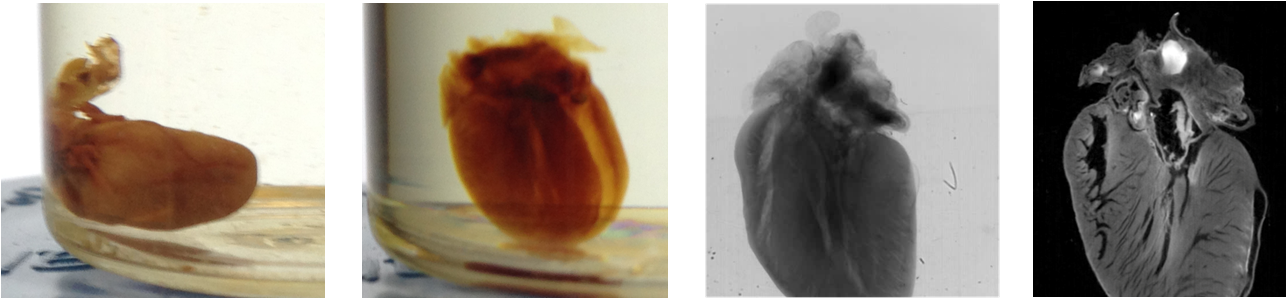
\includegraphics[width = \textwidth]{clearing_process_heart.png}}
		%	\subfigure[Clearing brain]{\label{subfig:clearingbrain}
		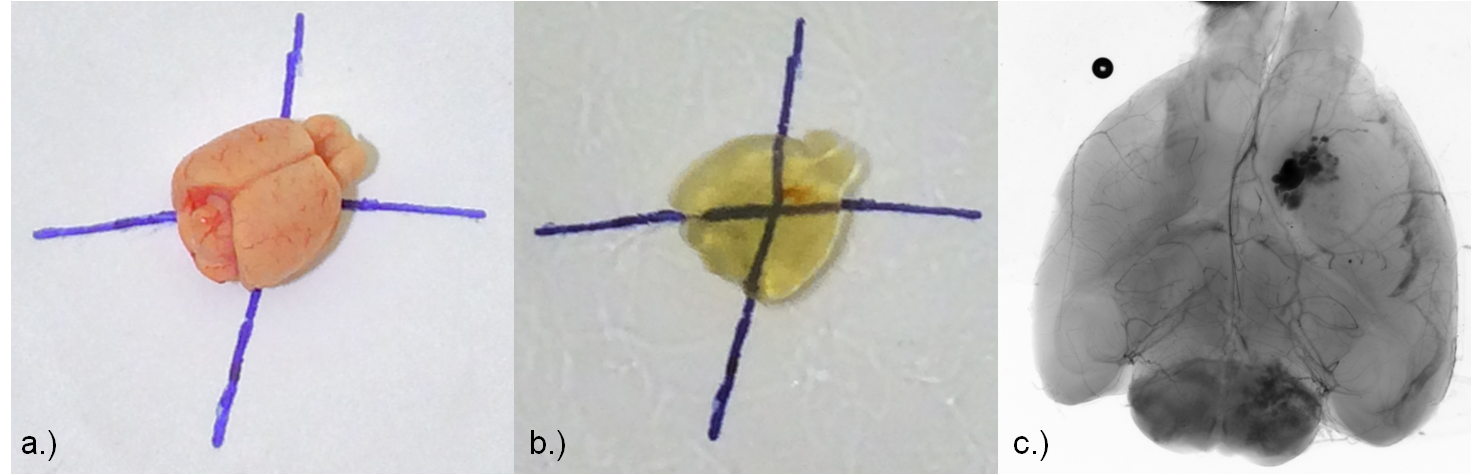
\includegraphics[width = \textwidth]{meth_img/Brain_J5_clearing.png}
		\caption{a. Example of an uncleared mouse brain, b. a cleared mouse brain in 1:2 BABB solution, c. a projection image of the cleared brain mounted in the optical CT system.}
		\label{fig:clearing}
	\end{figure}




%\begin{figure}[H]
%	\centering
%	\subfigure[System setup photo]{\label{subfig:tissuesetupphoto}
%		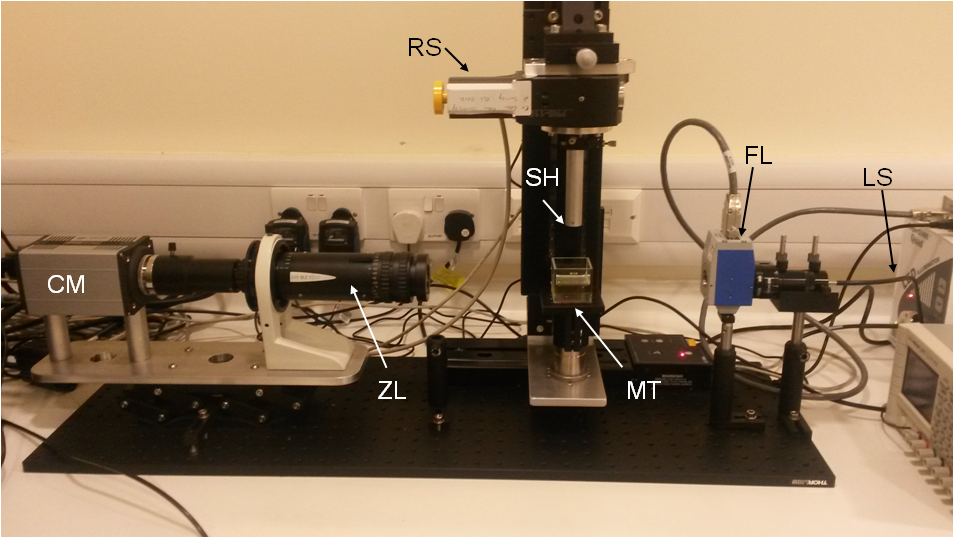
\includegraphics[width = 0.85\textwidth]{Tissue_set-up.png}}
%	\caption{Diagram and picture  of current set-up of tissue OptCT system at the ICR with principal parts of apparatus labelled. Add pictures of sample preparation.}
%	\label{fig:tissuesetup_pic}
%\end{figure}



Examples images of different healthy rodent organs are shown in Figure~\ref{fig:heart_brain}. Clearing with BABB has worked well and all contrast is endogenous. Clearing reduces light attenuation due to scattering, so any contrast is due to natural differences in light absorption properties between different tissue types. Highly attenuating areas, such as haemoglobin in the heart, or lipid-dense areas of the brain, are bright in these optical CT absorption scans.

%Images of tissues containing tumours are shown in Figure~\ref{fig:tumours}, ranging from a large neuroblastoma tumour, of the order of 10mm, to a tumour cell spheroid around $100\mu$m diameter, at the extreme resolution limit of the system. It was noted that large and highly attenuating tissues (such as neuroblastoma tumours) required longer clearing time.


	\begin{figure}[H]
		\centering
		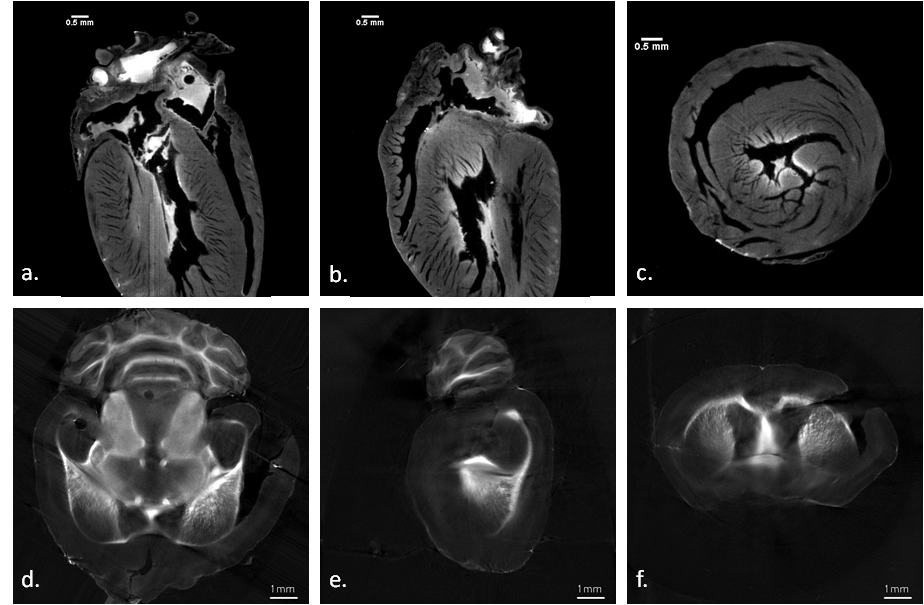
\includegraphics[width = \textwidth]{meth_img/heart_brain_sclbr.png}
		\caption{a-c.) Orthogonal slices of a reconstructed image volume of a mouse heart with endogenous contrast, most likely due to the presence of haemoglobin. d-f.) Orthogonal slices of a reconstructed image volume of a mouse brain where bright areas are likely due to attenuation due to lipid content of the brain. These images demonstrate high-resolution, highly detailed data reconstructed from absorption optical CT scans,  without addition of external contrast.}
		\label{fig:heart_brain}
	\end{figure}
	
%	\begin{figure}[H]
%		\centering
%		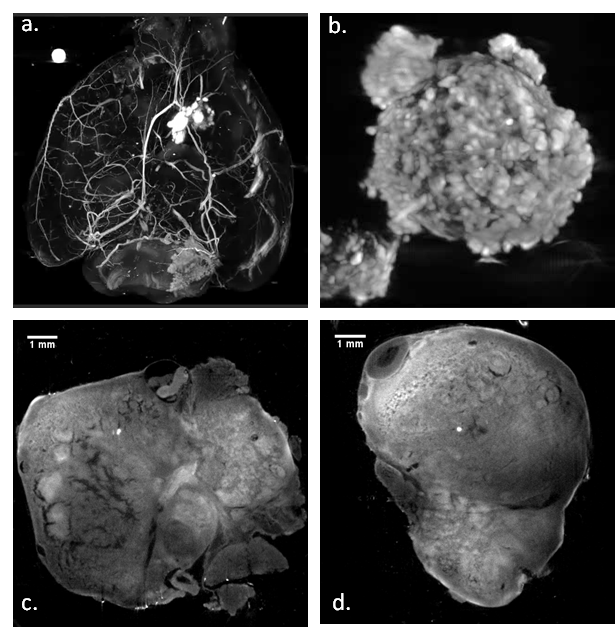
\includegraphics[width = \textwidth]{meth_img/tumours.png}
%		\caption{a.) Maximum intensity projection (MIP) of a mouse brain with an orthotopic glioblastoma tumour. A highly attenuating artefact due to an air bubble is seen in the top left corner. The mouse was injected with Evans Blue, an absorbing permeability marker which has stained the vasculature. The tumour was rich in haemoglobin and also appears very attenuating. This shows the potential for optical CT imaging of vasculature. b.) MIP image of a tumour cell spheroid stained with haematoxylin. c-d.) Orthogonal slices through a neuroblastoma tumour showing the detail possible using an anatomical scan. Additional functional information can be added with the use of fluorescent markers. }
%		\label{fig:tumours}
%	\end{figure}









\section{Optical CT system characterisation}

\subsection{Linear response}

In order to establish the relationship between optical CT reconstructed pixel value and optical absorbance,  gel finger phantoms were made in a similar fashion to \cite{Oldham:2003}.  


A specialised finger phantom mould was made by the ICR workshop. A 3-D printed plastic mould contained three removable metal rods on one side and an attachment for the rotation stage on the other. 
%A cylinder of Teflon FEP heat-shrink plastic (Holscot Fluoroplastics Limited, Grantham, UK) was used to provide support for the gelatin. Teflon FEP has an RI of 1.341  making it a very close match for water and gelatin. \cite{Krstajic:2006kna} 
Cylindrical pieces of Teflon FEP sleeving (RI 1.341, Holscot Fluoroplastics Limited, Grantham, UK) were cut a length of 4 cm, the height of the matching tank and one end was heat shrunk onto the plastic mould providing a secure support for the cooling gelatin. A small gap between the Teflon sleeve and the mould was left to allow airflow, meaning the metal rods can be removed easily. 

 
Clear gelatin (10\% porcine gelatin (G2500, Sigma-Aldrich) in water) was allowed to set at room temperature around the metal rods, which  were then carefully removed.  Evans Blue (T-1824), an azo dye which is both optically absorbing and  fluorescent, was used to provide optical contrast. Small amounts of Evans blue were added progressively to gelatin which was kept at $30^{\circ}$C using a heater-stirrer. The Evans blue-doped gelatin was injected into inclusions left by the metal rods using a 1 ml syringe. A cuvette of each concentration of Evans blue gelatin  was filled and allowed to set. The optical absorbance of each cuvette was measured using a spectrophotometer. Two phantoms were made in this manner, phantom A had 3 mm diameter inclusions and phantom B had 2 mm inclusions, with increasing Evans Blue concentrations.

The phantoms were scanned under the same imaging conditions. The matching liquid used was 4.5\% salt solution (RI $\approx 1.341$) which  gives a closer refractive index  match to Teflon FEP than water. The average reconstructed pixel value of each finger was calculated from a single axial slice and averaged over a $25 \times 25$ pixel area within the inclusion (see Figure~\ref{fig:fingerphantoms_roi_EB}b).
As can be seen in Figure~\ref{fig:fingerphantoms_roi_EB}c, the reconstructed pixel value of the optical CT system is linearly related to the optical absorbance as measured by  spectrophotometer.   The use of two phantoms verifies the linear relationship and the repeatability of measurements.  

	\begin{figure}[H]
		\centering
		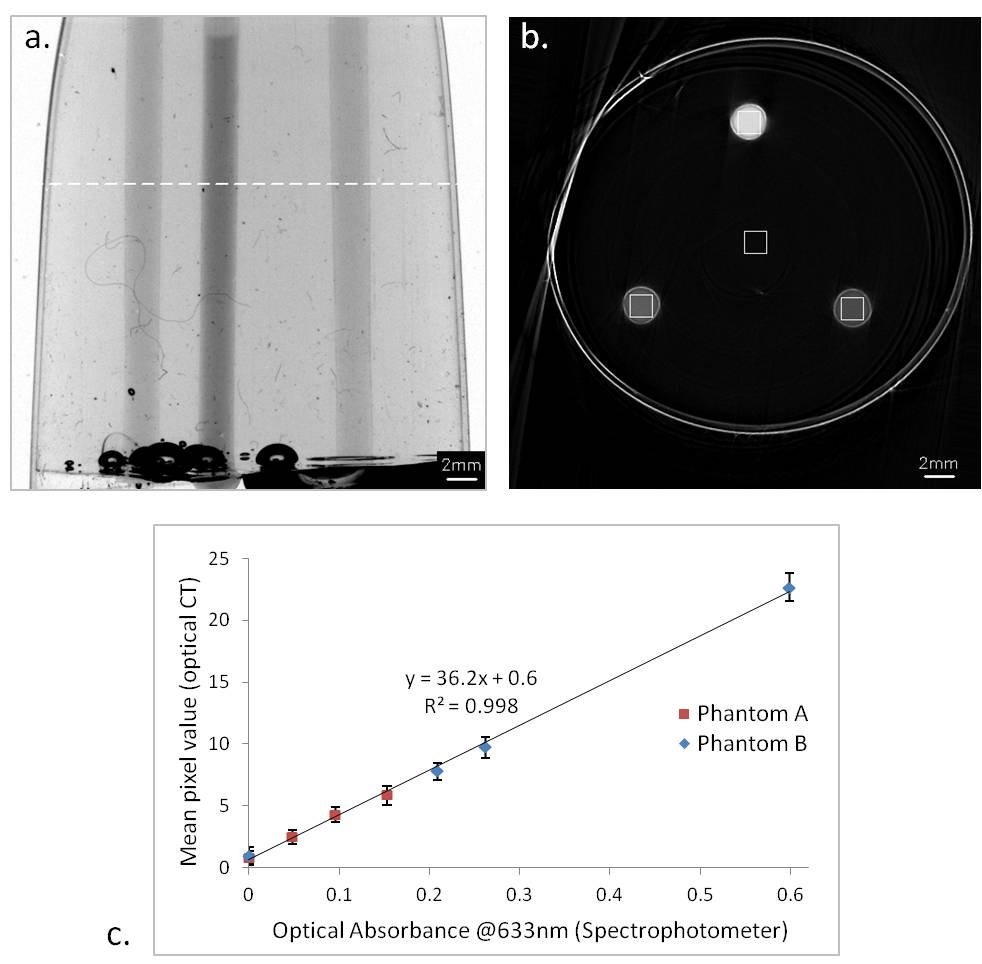
\includegraphics[width=1\textwidth]{meth_img/EB_rod_new.jpg}
		\caption{a. An optical CT projection image of a gelatin phantom containing `finger' inclusions of different concentrations of Evans blue-dyed gel. b. A reconstructed slice through the phantom in the axial position marked by the dashed line in (a). Regions of Interest (ROIs) mark where the mean pixel value was calculated for each finger and the clear gelatin. The double ring artefact is due to refractive index mismatch between gel and the Teflon FEP container, and also between the Teflon and 4.5\% saline matching liquid. c. Plot of absorbance of Evans Blue-doped gel measured with a Spectrophotometer against mean pixel value of different regions on reconstructed optical CT images. Two phantoms were measured  with all  variables constant between readings.}
		\label{fig:fingerphantoms_roi_EB}
	\end{figure}
	








\subsection{Spatial resolution}
\label{subsec:spat_res}

Understanding the spatial resolution response of the optical CT system is very important for acquiring high-quality, quantitative images. There are many factors which can affect optical CT resolution (see theory section?).
Previous publications noted a reduction of optical CT image contrast of small features as the feature size approaches the resolution. \cite{doranultra-high2013} This effect is evident even when the feature size is several times the nominal spatial resolution and leads to non-linear response to optical absorbance. Therefore, the limits of spatial resolution of the system must be carefully characterised before we can be confident that measurements are quantitative. 

% as ideally the entire sample should be in focus at all times (see Figure~\ref{fig:idealdof}). 
For optical CT the spatial resolution either side of the focal plane along the optical axis is important. The distance over which the focus is `acceptable' is known as the depth-of-field (DOF).
Ideally the DOF of projection images should be larger than or equal to the sample size, as demonstrated in Figure~\ref{fig:idealdof}. However, there is a trade-off between DOF and spatial resolution,  $\Delta x$, given by \cite{inoue1997video} as follows,
\begin{equation}
\mathrm{DOF} = \frac{n_{bath}}{0.61 n \lambda} \big(\Delta x^2 + \frac{ne}{\mathrm{M_{lat}}} \Delta x \big)
\label{eqn:1DOF}
\end{equation}
where, $n_{bath}$ is the refractive index of the medium surrounding the sample, $n$ is the refractive index of the medium around the lens, $\lambda$ is the wavelength of light, $e$ is the pixel size of the camera and $\mathrm{M_{lat}}$ is the lateral magnification of the system. The DOF of the system can be adjusted by adjusting an aperture in the lens system. This adjusts the overall acceptance angle of the system, $\theta$, which in turn controls the numerical aperture (NA), which is inversely proportional to the resolution and DOF.
\begin{equation}
\mathrm{NA} = n \sin \theta = \frac{0.61n\lambda}{\Delta x}
\label{eqn:2NA}
\end{equation}


%The optical system consists of components from a modular microscope system. This includes a zoom lens, giving variable magnification settings, and a variable aperture which controls the DOF of the system. 
%The aperture size can determine the overall acceptance angle of the optical system, $\theta$, which in turn affects the numerical aperture (NA), defined as $N_A = n \sin{\theta}$.  A system with high NA results in high resolution, $\Delta x$ (Equation~\ref{eqn:airy}). However, such a system has a small DOF due to the inverse relationship between DOF and NA (Equation~\ref{eqn:dof}).
%\begin{equation}
%\Delta x =  \frac{0.61 n\lambda}{N_A}
%\label{eqn:airy}
%\end{equation}
%\begin{equation}
%\mathrm{d_{DOF}} = n_{bath}\left( \frac{n\lambda}{N_{A}^2}+\frac{ne}{MN_{A}} \right) = \frac{n_{bath}}{0.61n\lambda}\left( \Delta x^2 + \frac{n e}{M}\Delta x \right)
%\label{eqn:dof}
%\end{equation}
%where $n$, the refractive index of the medium around the lens, $n_{bath}$ the refractive index of the medium surrounding the sample, $M$ the lateral magnification of the system, $e$ the pixel size of the camera and $\lambda$, the wavelength of light.



\begin{figure}[H]
	\centering
	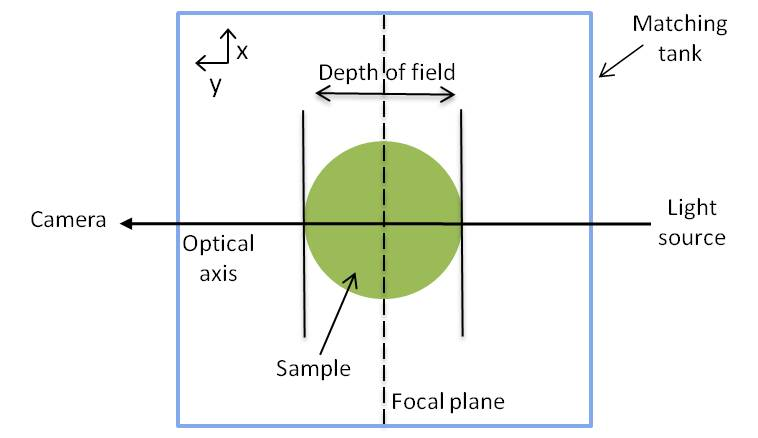
\includegraphics[width=0.9\linewidth]{meth_img/ideal_dof_diagram}
	\caption{Schematic of the optical CT system geometry showing the ideal positions of the focal plane and depth-of-field.}
	\label{fig:idealdof}
\end{figure}



To investigate the effect of changing the NA of our system we measured the modulation transfer function (MTF) for a range of positions along the optical axis. Five different NA values were evaluated, corresponding to the five reproducible aperture size settings on the lens system, labelled as A1 to A5, with A1 being the smallest aperture and A5 being the fully open aperture setting, with the largest NA. 

The modulation transfer function (MTF) characterises the resolution of a system by measuring how different spatial frequencies are transmitted.
It is the Fourier transform of the Point Spread Function (PSF), giving a more comprehensive description of an optical system than quoting a single  resolution value. There are various methods of measuring the MTF, including simulating a point source or measuring the response to a sinusoidal pattern. These methods require test objects accurate to sub-pixel distances. 
It is much easier to manufacture an accurate  sharp edge rather than  a point source or slit. It has been shown that the MTF can be calculated analytically from the Edge Spread Function (ESF) as follows,
\begin{equation}
\mathrm{MTF}(f) = \mathscr{F}\left[\mathrm{LSF}(x)\right] = \mathscr{F}\left[\frac{d}{dx}\mathrm{ESF}(x)\right]
\label{eqn:MTF_ESF}
\end{equation}
where $f$ is spatial frequency, $x$ is displacement and LSF is the Line Spread Function given by the profile of a slit source. \cite{Boone:1986}

%Any noise in the data is amplified  through the derivative and Fourier transform. Therefore, following the method of Boone \textit{et al.},   the MTF was calculated directly from the fit parameters of a function  fitted directly to measured ESF data. \cite{Boone:1994} Analysis was carried out in IDL  using curve fitting function `\textit{mpfit}'.  \cite{Markwardt2009mpfit}

A knife edge was positioned at the focal plane and 50 projection images of matrix size $2048 \times 2048$ were acquired and averaged to improve the signal-to-noise ratio (SNR). The knife edge was moved in steps of 0.1 mm away from the focal plane in both directions along the optical axis.  Images were acquired over a distance of 0.5 mm in each direction giving a total distance of 1 mm, the same as the FOV of each projection image. This was repeated for each aperture setting of the microscope lens.


%Plotting the MTF at each position along the optical axis as an image, the DOF is visualised in a similar manner to  \cite{chenincorporation2012}. The maximum resolution for each NA was taken as the largest spatial frequency with continuous MTF values over 0.1 over some y-range, being the DOF for that resolution.

%The MTF was calculated from ESF data, as seen in Figure~\ref{fig:MTFtarget},  for a range of magnifications, pixel binning and LED voltages. The results  in Figures~\ref{fig:MTF_50}  show that system response varies significantly with these variables as is expected. Magnifcations of 0.8, 1 and 8 were tested to demonstrate the worst,  standard and best conditions for imaging respectively.



The MTF was calculated from the ESF, measured across the centre of the knife-edge images, according to equation~\ref{eqn:MTF_ESF} for each position along the optical axis and for each NA value. The MTF was represented by a grey level in a 2-D image in which the horizontal coordinate corresponds to spatial frequency, up to the desired 100 mm$^{-1}$ (equivalent to a $10 \mu$m line-pair), and the vertical coordinate corresponds to position along the optical axis (see Figure~\ref{fig:MTFDOF}). This allows visualisation of the DOF for each of the different NA values.

The maximum resolution and corresponding DOF were measured for each NA setting. The maximum resolution was defined as the largest spatial frequency with an MTF above 10\% at the focal plane. The DOF for this frequency was defined as the distance along the optical axis for which this spatial frequency had an MTF above 10\%.  
The observed DOF and resolution results are shown in Table~\ref{table:DOFNA}.
It is apparent that for low NA, there is a constant, low resolution across the entire FOV whereas at high NA there is a small region of high-resolution with other areas being defocused. 
%NA values in between show a sharp drop-off of DOF.


%	\begin{figure}[H]
%		\centering
%		\subfigure[`Knife-Edge' Target]{\label{subfig:MTFtarget}
%			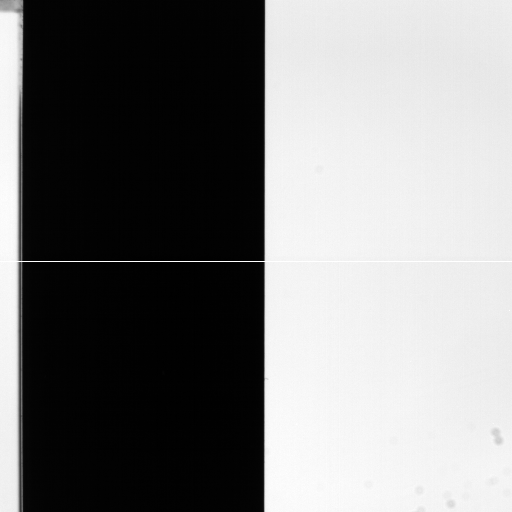
\includegraphics[width=0.3\linewidth]{meth_img/MTF3_targetimage.png}}
%		\subfigure[Edge spread function from image \ref{subfig:MTFtarget}]{\label{subfig:ESF}
%			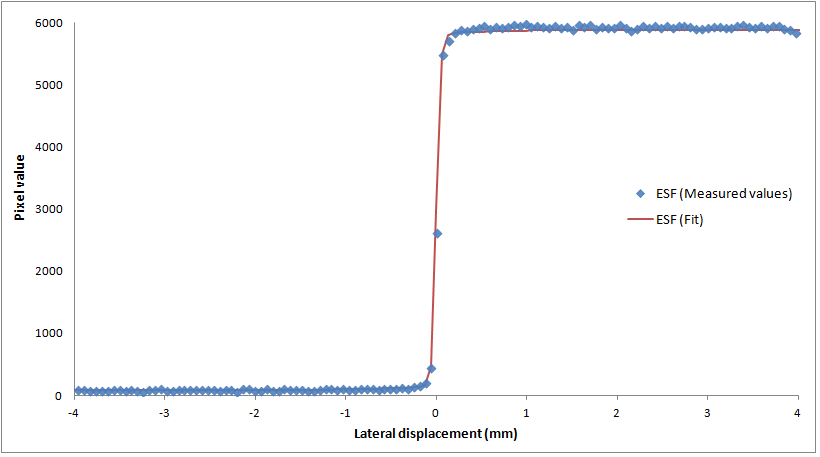
\includegraphics[width=0.55\textwidth]{meth_img/croppedESF_MTF3.png}}
%		\caption{Image of a rectangular metal target with a straight edge which  approximates a `Knife' edge for the measurement of the Edge Spread Function (ESF, \ref{subfig:ESF}). The pixel row across which the ESF is measured is marked on the image. This data was cropped to give 300 points centred on the edge to allow a curve to be fitted to the data  accurately.  Pixel size was measured  allowing the pixel values to be plotted against displacement. The point of zero displacement was set at the edge for convenience in fitting a curve to the data.  The MTF is calculated directly from the ESF via  fit parameters. }
%		\label{fig:MTFtarget}
%	\end{figure}

	\begin{figure}[H]
		\centering
		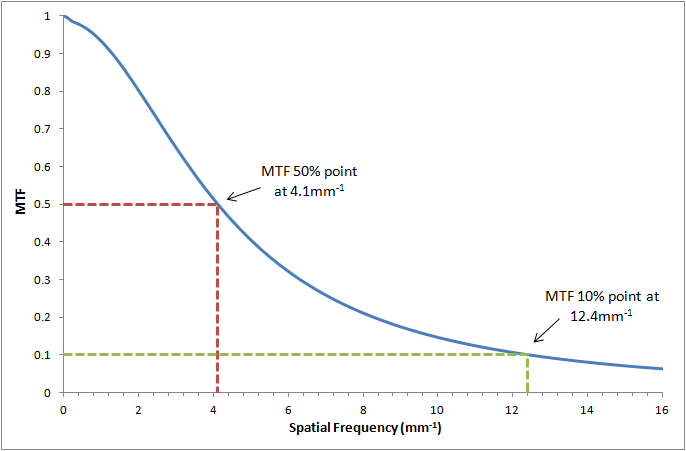
\includegraphics[width = 0.7\textwidth]{meth_img/MTF_50_graph.png}
		\caption{MTF vs spatial frequency for the case of M=1, $4 \times 4$ binning to 512x512 pixels and  LED voltage set to just below camera saturation levels, representing the imaging conditions  for most phantom images in this report. The 50\% cut-off point for the MTF, a value commonly quoted as giving the best focus is found to be 4.1 mm$^{-1}$. The 10\% MTF value is 12.4 mm$^{-1}$ and in general this value indicates the highest  frequency that can be resolved by the system. This implies that features smaller than $40 \mu$m will not be resolved at this magnification and binning. CHANGE GRAPH, INLCUDE FOCAL PLANE AND AWAY COMPARISON}
		\label{fig:MTF_50}
	\end{figure}




These results indicate that aperture settings must be chosen carefully for each imaging application. For most cases a constant resolution across the FOV is desirable, therefore A1 is appropriate. For some cases, it may be desirable to have very high resolution in a small area around the centre of rotation in which case a higher aperture setting may be appropriate. 
These measurements were all taken in `projection' space and do not take into account the effect of the reconstruction process on resolution. 




	\begin{figure}[H]
		\centering
		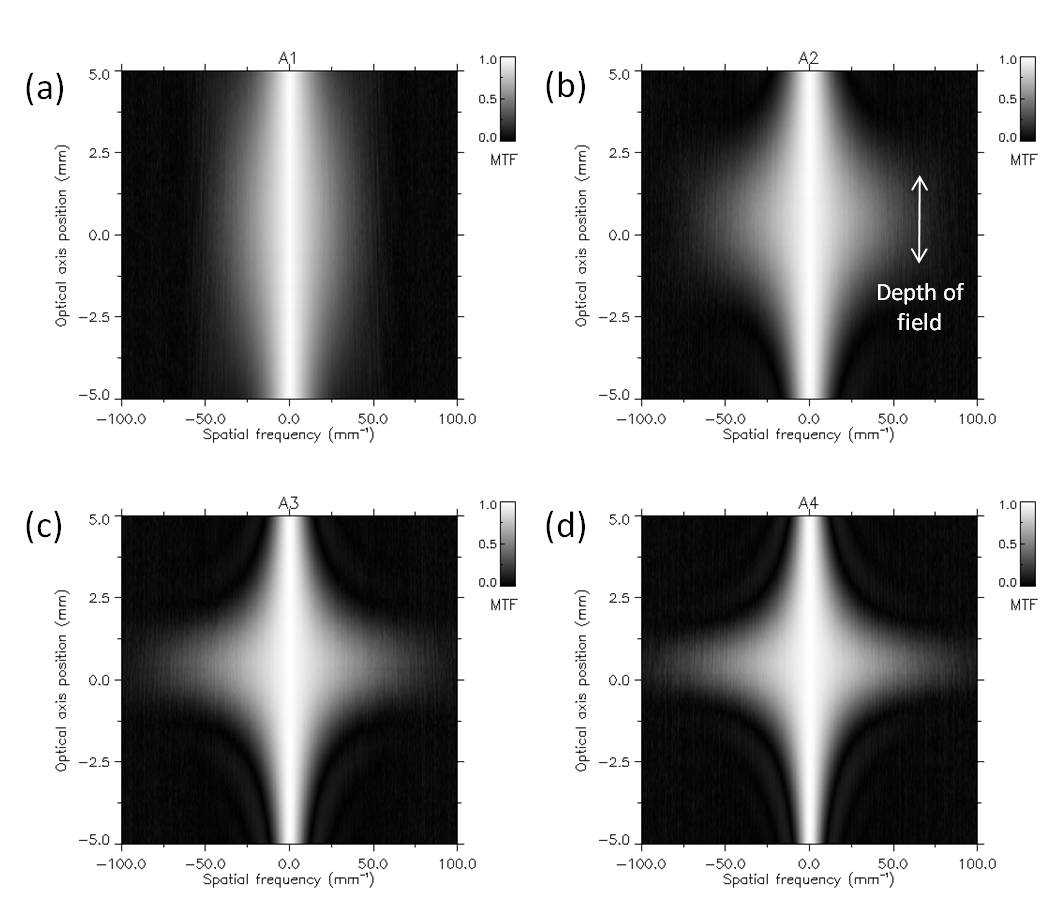
\includegraphics[width=0.9\linewidth]{mrt_img/mrt_Fig6}
		\caption{Measurements of the modulation transfer function (MTF) along the optical axis for different numerical aperture (NA) settings of the system, (a) A1 (b) A2 (c) A3 (d) A4. This allows visualisation of the depth-of-field (DOF).}
		\label{fig:MTFDOF}
	\end{figure}
	
	\begin{table}[H]
		\centering
		\begin{tabular}{ p{2.5cm} p{1.8cm} p{3cm} p{3cm}  }
			\hline
			\textbf{NA setting} & \textbf{NA} & \textbf{Resolution ($\mu$m)} &\textbf{Depth of field (mm)}  \\ \hline
			A1  & 0.0086 & $21.5 \pm 0.5$ & $9.3 \pm 0.4$ \\ %\hline
			A2  & 0.0155 & $13.7 \pm 0.1$ & $2.4 \pm 0.2$ \\ %\hline
			A3  & 0.0204 & $12.0 \pm 0.2$ & $1.6 \pm 0.2$ \\ %\hline
			A4  & 0.0252 & $10.1 \pm 0.2$ & $0.6 \pm 0.1$ \\ %\hline
			A5  & 0.0290 & $9.7  \pm 0.2$ & $0.4 \pm 0.1$ \\ \hline		
		\end{tabular}
		\caption{Maximum resolution and corresponding depth-of-fields for different NA settings on the optical CT system. The uncertainties reflect noise in the modulation transfer function (MTF)  measurements.}
		\label{table:DOFNA}
	\end{table}





\subsection{Focal position}
\label{sec:focalpos}

Positioning of the focal plane is very sensitive,  illustrated through the use of a `point' object test phantom containing $5 \mu$m beads. As seen in Figure~\ref{fig:bead_DOF}, a small displacement of the focal plane from the centre of the sample gives uneven focus. 

A bead phantom was made, optical axis stage adjusted until in the middle of FOV.  etc

It is possible to attach this  bead phantom to the bottom of other samples which gives us the ability to quantify  how the resolution changes over the FOV. 


Bead phantom construction. A5, m=8, sum 50 slices to get good visualisation

\begin{figure}
\centering
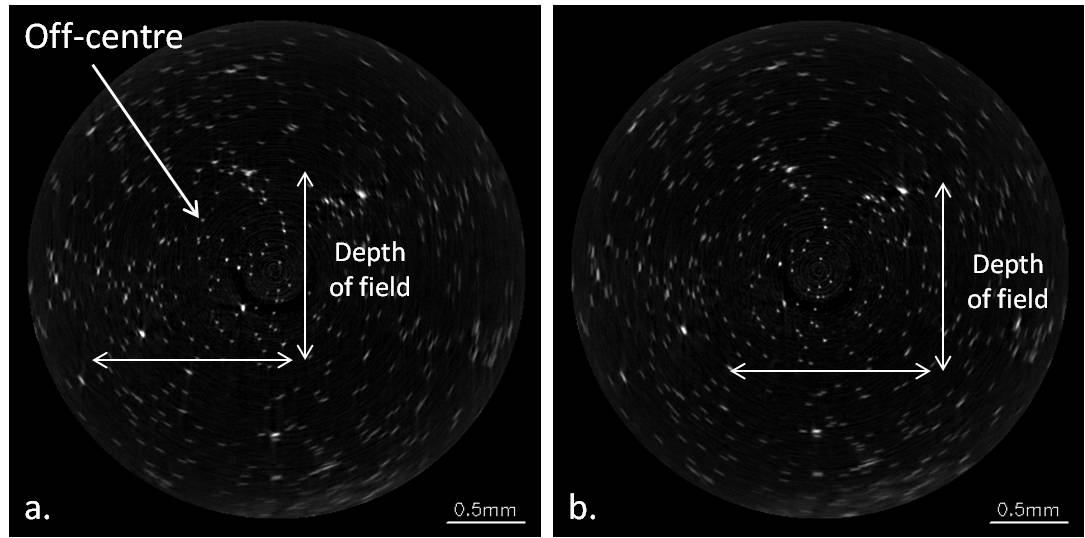
\includegraphics[width=\linewidth]{meth_img/focusing_beads.jpg}
\caption{a. Bead image with optical axis position ? showing unsymmetrical focus b. corrected focal plane, central focus.}
\label{fig:bead_DOF}
\end{figure}



\section{Conclusions}

The optical CT system has been developed, increase in speed of acquisition with new hardware and acquisition protocol. Adaptations to allow tissue imaging have been made and a tissue sample preparation process has been established. 

The system has been thoroughly characterised which is important before quantitative measurements can be made. The linearity has been established and the spatial resolution characterised for different settings. These results will be used to help make informed choices on the optimal scanning parameters for future samples. 

















